%%%%%%%%%%%%%%%%%%%%%%%%%%%%%%%%%%%%%%%%%%%%%%%%%%%%%%%%%%%%%%%%%%%%%%%%%%%
%
% Plantilla para un artículo en LaTeX en español.
%
%%%%%%%%%%%%%%%%%%%%%%%%%%%%%%%%%%%%%%%%%%%%%%%%%%%%%%%%%%%%%%%%%%%%%%%%%%%



%--------------------------------------------------------------------------
\title{Plantilla para un artículo \LaTeX}
\author{El autor va aquí\\
  \small Dept. Plantillas y Editores\\
  \small E12345\\
  \small España
}

\begin{document}
\maketitle

\abstract{Esto es una plantilla simple para un artículo en \LaTeX.}
\\
\abstract{Esto es una plantilla simple para un artículo en \LaTeX.}

\section{Introduccion}

Aquí va el texto.
\begin{equation}\label{eq:area}
  S = \pi r^2
\end{equation}
Uno puede referirse a ecuaciones así: ver ecuación (\ref{eq:area}).
También se pueden mencionar secciones de la misma forma: ver sección
\ref{sec:nada}. O citar algo de la bibliografía: \cite{Cd94}.

\section{Marco teorico}
\title{BUSINESS INTELLIGENCE}\\\\
La Inteligencia de Negocios BI (Business Intelligence) es una herramienta bajo la cual diferentes tipos de organizaciones, pueden soportar la toma de decisiones basadas en información precisa y oportuna; garantizando la generación del conocimiento necesario que permita escoger la alternativa que sea más conveniente para el éxito de la empresa.\\\\
\begin{figure}[htb]
\begin{center}

\includegraphics[width=10cm]{./Imagenes/inegocios}
\end{center}
\end{figure}
Desde un punto de vista más pragmático, y asociándolo directamente con las tecnologías de la información, podemos definir Business Intelligence como el conjunto de metodologías, aplicaciones y tecnologías que permiten reunir, depurar y transformar datos de los sistemas transaccionales e información desestructurada (interna y externa a la compañía) en información estructurada, para su explotación directa (reporting, análisis OLTP / OLAP, alertas...) o para su análisis y conversión en conocimiento, dando así soporte a la toma de decisiones sobre el negocio.\\\\
Los principales productos de Business Intelligence que existen hoy en día son:

*  Cuadros de Mando Integrales (CMI)

*  Sistemas de Soporte a la Decisión (DSS)

*  Sistemas de Información Ejecutiva (EIS)
\\\\
\title{BUSINESS ANALYTICS}\\\\
El análisis de negocio(Business Analytics, BA) es el conjunto de métodos y técnicas utilizadas para trabajar como enlace entre los stackeholders, con el fin de comprender la estructura, políticas y operaciones de una organización y recomendar soluciones que permitan a la organización alcanzar sus objetivos (IIBA: International Institute of Business Analysis).\\\\
El análisis de negocios implica la comprensión de cómo funcionan las organizaciones para llevar a cabo sus propósitos, y la definición de las capacidades que una organización requiere para proporcionar productos y servicios a los grupos de interés externos. Incluye la definición de los objetivos de la organización, cómo esos objetivos se conectan a objetivos específicos, que determinan las líneas de acción que una organización tiene que realizar para alcanzar esas metas y objetivos, y definir cómo las distintas unidades de organización y las partes interesadas dentro y fuera de esa organización interactúa.

\begin{figure}[htb]
\begin{center}
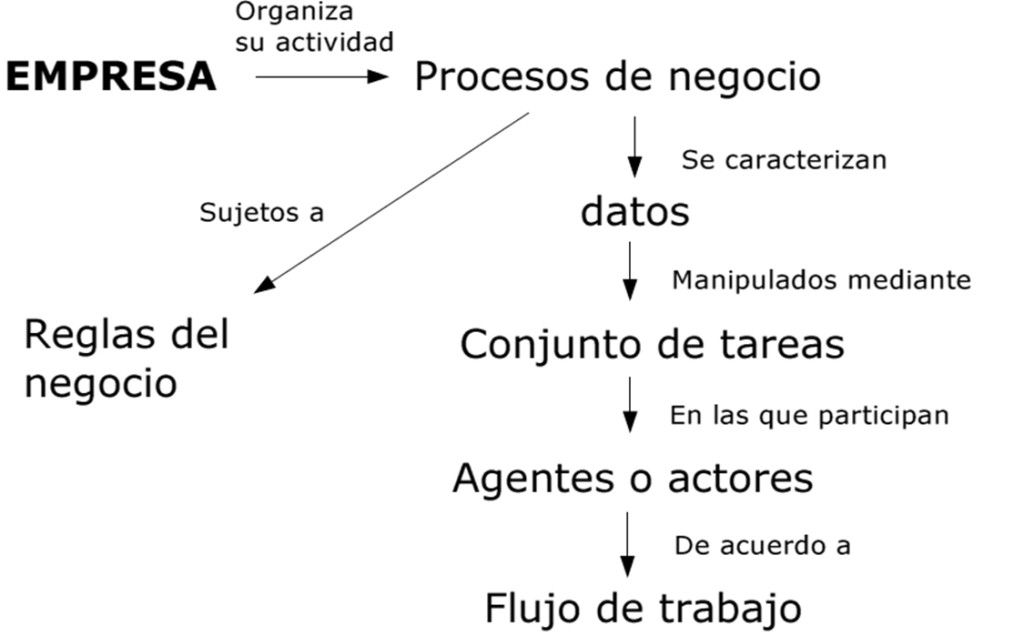
\includegraphics[width=10cm]{./Imagenes/anegocios}
\end{center}
\end{figure}

\section{Aplicacion}

Aquí va el texto.
\begin{equation}\label{eq:area}
  S = \pi r^2
\end{equation}
Uno puede referirse a ecuaciones así: ver ecuación (\ref{eq:area}).
También se pueden mencionar secciones de la misma forma: ver sección
\ref{sec:nada}. O citar algo de la bibliografía: \cite{Cd94}.



\subsection{Aplicaciones de BuBusiness Intelligence } \label{sec:nada}
\subsection{Subsection}\label{sec:nada}

Las herramientas de inteligencia de negocio son aplicaciones digitales diseñadas para colaborar con el Business Intelligence durante el análisis y la presentación de datos.\\
La Inteligencia de Negocios o Business Intelligence (BI) permite a las compañías contar con la información adecuada para una mejor toma de decisiones.  Las compañías que implementan el BI logran sacar mayor provecho de las situaciones de crisis gracias a la posibilidad de contar con un análisis de mercado más acertado debido a que los datos pesados son transformados en importantes estrategias corporativas.
Actualmente, las herramientas de BI disponibles en el mercado son incontables, pero estas 20 no pueden pasar desapercibidas:

\subsubsection{Subsubsection}\label{sec:nada2}

Más texto.


\section{Conclusiones}

(\ref{eq:area}).
También se pueden mencionar secciones de la misma forma: ver sección
\ref{sec:nada}. O citar algo de la bibliografía: \cite{Cd94}.


% Bibliografía.
%-----------------------------------------------------------------
\begin{thebibliography}{99}

\bibitem{Cd94} Autor, \emph{Título}, Revista/Editor, (año)

\end{thebibliography}

\end{document}
